\documentclass[a0,landscape]{a0poster}

\usepackage{mathtools,natbib,graphicx,tcolorbox,float,newtxtext,newtxmath} %packages (incl. alternate math fonts)
\usepackage{multicol} % This is so we can have multiple columns of text side-by-side
\columnsep=1cm % This is the amount of white space between the columns in the poster
\columnseprule=0pt % This is the thickness of the black line between the columns in the poster
\usepackage{tabularx}
\setlength{\tabcolsep}{1cm}
\renewcommand{\arraystretch}{1}
\renewcommand{\familydefault}{\sfdefault} %set sans-serif font
\setlength{\bibsep}{0.0pt}   %close bibliography entries
\floatplacement{figure}{H} %force figure placement in section
\usepackage{braket}
\usepackage{amsfonts}
\usepackage{subcaption}
\usepackage{algorithm}
\usepackage{placeins}
%\usepackage{algorithmic}
\usepackage[noend]{algpseudocode}
\usepackage[export]{adjustbox}
\usepackage{xcolor,colortbl}


\begin{document}

\pagecolor{gray!25} %set background
\tcbset{left=30pt,right=30pt,top=30pt,bottom=30pt, colback=white,colframe=black,title=\textcolor{white}, toptitle=0.2cm, bottomtitle=0.2cm} %set tcolorbox defaults (can change individual boxes still)

% TOP BAR
\begin{minipage}[t]{0.2\linewidth}
\begin{figure}
  \centering
  \includegraphics[width=0.8\linewidth]{VSLogo.pdf} 
\end{figure}
\end{minipage}
%
\begin{minipage}[t]{0.60\linewidth}
\begin{center}
\color{white}
\Huge \color{black}  \textbf{\textsf{Efficient Near-Optimal Multi-Qubit Clifford + T Gate Synthesis\\}} 
\huge \textsf{\underline{\smash{Luke E. Heyfron}\textsuperscript{*}} and Earl T. Campbell$^\dagger$}\\  \Large
\vspace{0.5cm}Department of Physics and Astronomy, The University of Sheffield \\ \textsuperscript{*}\textit{leheyfron1@sheffield.ac.uk}, $^\dagger$\textit{e.campbell@sheffield.ac.uk}
\end{center}
\end{minipage}
%
\begin{minipage}[t]{0.2\linewidth}
\begin{figure}
\includegraphics[width=0.8\linewidth]{EPSRClogoB.pdf} 
\end{figure}
\end{minipage}
%

\vspace{1cm}

\normalsize

\begin{multicols}{3}
		
	% LEFT COLUMN
	
	\begin{minipage}[b]{\linewidth}
		% INTRODUCTION
		\begin{tcolorbox}[title=\textcolor{white}{\huge\textbf{\textsf{Introduction}\textcolor{black}{y}}}]
			\iffalse The objective is to reduce cost of quantum circuits.
			Quantum circuits break down complex algorithms into elementary steps or gates.
			The cost of each gate must take into account effects of noise.
			Noise mitigated by QEC codes.
			Gates must act on encoded states to remain protected.
			Only some natively protected gates - Clifford gates for high threshold codes.
			T gates allow for universal QC but require extra gadgets and magic state distillation to be fault tolerant and therefore are considered an expensive resource in the magic states model of QC.
			Gate synthesis aims to generate circuit decompositions for some target unitary that uses minimal T gates.
			Optimal algorithm is computationally inefficient so important to find fast near optimal algorithms. \fi
			%
			Quantum computers are expensive to run in practice, motivating us to minimize the amount of time and space resources consumed by executing quantum algorithms. Quantum circuits allow us to decompose complex quantum algorithms into elementary quantum gates. However, the cost of each gate is not necessarily uniform - rather we must take into consideration the quantum error correction (QEC) code used to protect our quantum memory from noise. High-threshold codes such as the 2D surface code \cite{29_Dennis_2002} only natively support a limited set of operations, requiring expensive extra steps to realise universal quantum computation. The magic states model \cite{32_Bravyi_2005} is one of the leading proposals for fault-tolerant quantum computations and assumes that so called Clifford operations are free and implies that the cost of a circuit is proportional to the number of uses of the $T$ gate, or the $T$-count of a circuit. We consider the gate synthesis problem of finding circuit decompositions with minimal T count that implement a given $n$ qubit unitary generated by the Clifford + T gate set. There are no known optimal solvers for this problem that are computationally efficient in the number of qubits. Moreover, the problem is believed to be hard. Therefore, it is desirable to develop efficient algorithms that yield near-optimal solutions. To this end, we present an efficient near-optimal T gate optimization algorithm that yields lower T counts than the best known previous algorithms, which we have implemented in C++ along with competing algorithms.
			%
			\iffalse Quantum computers are able to solve certain problems much faster than classical computers, as is well demonstrated by Shor's factoring \cite{24_Shor_1999} and Grover's search algorithm \cite{grover_1996}. But running a quantum computer is expensive in practice, motivating us to minimize the amount of time and space resources consumed by executing quantum algorithms. Quantum circuits allow us to decompose complex quantum algorithms into elementary quantum gates. However, the cost of each gate is not necessarily uniform - rather we must take into consideration the quantum error correction (QEC) code used to protect our quantum memory from noise. High-threshold codes such as the 2D surface code \cite{29_Dennis_2002} only natively support a limited set of operations, requiring expensive extra steps to realise universal quantum computation. The magic states model \cite{32_Bravyi_2005} is one of the leading proposals for fault-tolerant quantum computations and assumes that so called Clifford operations are free and that the cost of a circuit is proportional to the number of uses of the T gate, or the T count of a circuit. This model presents the \textbf{gate synthesis problem} of finding circuit decompositions with minimal T count that implement a given unitary generated by the Clifford + T gate set. There are no known optimal solvers for this problem that are computationally efficient in the number of qubits. Furthermore, the problem is believed to be hard. Therefore, it is desirable to develop efficient algorithms that yield near-optimal solutions. To this end, we present an efficient near-optimal T gate optimization algorithm that yields lower T counts than the best known previous algorithms, which we have implemented in C++ along with the competing algorithms. \fi
		\end{tcolorbox}
	
		% MAGIC STATES MODEL/MOTIVATION	
		 \iffalse \begin{tcolorbox}[title=\textcolor{white}{\huge\textbf{\textsf{Motivation}\textcolor{black}{y}}}]
			\iffalse Fault-tolerant quantum computation
			\iffalse Transversal gates: Clifford operations are cheap
			Non-transversal gates: Magic state distillation+injection expensive for the same precision.
			Gate synthesis problem is to find a circuit decomposition for an input unitary that has minimal uses of the T gate. \fi
			Our algorithm assumes that Clifford operations are free and that only the T gate contributes to the cost of the circuit but why?\fi
			%
			Both the Clifford operations and the T gate are required to form a universal gate set. However, for many QEC codes Clifford operations are \textbf{transversal}, whilst the $T$ gate is not. Transversal gates are natively protected by the QEC code and can be implemented in time proportional to the physical gate time, whereas non-transversal gate require magic state distillation and gate teleportation. 
			\iffalse For many QEC codes, Clifford operations are transversal, meaning they can be implemented by applying gate that act non-trivially on only a single qubit within the same code block and between corresponding qubits of different code blocks.
			Clifford operations alone are not sufficient for universal quantum computation, however, by adding the T gate, we get a universal gate set.
			For the same QEC codes, the T gate is not transversal so we must use a different approach to implement a T gate fault-tolerantly.
			The magic states model proposed Bravyi and Kitaev \cite{32_Bravyi_2005} allows us to implement the T gate by consuming a T-type magic state using a gate teleportation circuit.
			In order for the error rate of the T gate to be suppressed, the magic state must be of high fidelity.
			High fidelity magic states can be produced through magic state distillation protocols such as Bravyi and Haah's triorthogonal matrices that takes $3k+8$ noise magic states and outputs $k$ magic states with quadratically suppressed error.
			We can achieve error rates as low as $10^{-17}$ by performing distillation over several rounds, consuming several hundred raw input T states per output T state. \fi
			%			
			\iffalse The magic states model proposed Bravyi and Kitaev \cite{32_Bravyi_2005} assumes that Clifford operations can be performed perfectly and that we can prepare noisy ancilla states called magic states. High fidelity magic states can be produced by consuming raw noisy magic states in magic state distillation protocols such as the ``15-to-1'' Reed-Muller protocol; the ``10-to-2'' \fi
		\end{tcolorbox}\fi
	
		% DIAGONAL CNOT + T FRAMEWORK/THEORY
		\begin{tcolorbox}[title=\textcolor{white}{\huge\textbf{\textsf{Diagonal CNOT + T Framework}\textcolor{black}{y}}}]
			The action of any diagonal $n$ qubit unitary composed of only $\mathrm{CNOT}$ and $T$ gates, $U$, on a computational basis state, $\ket{\mathbf{x}}$, can be completely described by the \textbf{phase function} of $U$, $f:\mathbb{Z}_2^n \mapsto \mathbb{Z}_8$.
			\begin{equation*}
			U\ket{\mathbf{x}} = \omega^{f(\mathbf{x})}\ket{\mathbf{x}}
			\end{equation*}
			where $\omega = e^{i\frac{\pi}{4}}$.
			
			\iffalse The phase function has two kinds of decomposition of interest: the \emph{phase polynomial} and the \emph{weighted polynomial}. A phase polynomial for a given unitary corresponds to a particular circuit decomposition of that unitary, whereas the weighted polynomial is used to check that the unitary is the same after some transformation on the phase polynomial. \fi
			
			A \textbf{gate synthesis matrix}, $A$, is a streamlined representation of a circuit decomposition, $C$, that implements $U$ up to Clifford equivalence. Each column of $A$ corresponds to a single use of the $T$ gate (conjugated by some $\mathrm{CNOT}$ subcircuit); therefore, the number of columns of $A$ is equal to the $T$ count of $C$.							
			Furthermore, any two gate synthesis matrices with the same \textbf{signature tensor} implement the same unitary up to Clifford equivalence.
			It follows that the gate synthesis problem is to find the gate synthesis matrix with minimal number of columns that has the same signature tensor as some initial gate synthesis matrix that implements the input unitary.
			
			\vspace{1cm}
			\begin{tcolorbox}
				\iffalse\textbf{Phase Polynomial:}
				\begin{equation*}
				f(\mathbf{x}) = \sum_{t=1}^{N_t}m_t(A_{1,t}x_1 \oplus A_{2,t}x_2 \dots A_{n,t} x_n) \pmod{8}
				\end{equation*}
				
				\textbf{Weighted Polynomial:}
				\begin{equation*}
				f(\mathbf{x}) = \sum_{\alpha=1}^{n}l_{\alpha}x_{\alpha} + 2\sum_{\alpha<\beta}^{n}q_{\alpha,\beta}x_{\alpha}x_{\beta} + 4\sum_{\alpha<\beta<\gamma}^{n} c_{\alpha,\beta,\gamma}x_{\alpha}x_{\beta}x_{\gamma} \pmod{8}
				\end{equation*}\fi
			%\end{tcolorbox}
			%\begin{tcolorbox}				
				\textbf{Gate Synthesis Matrix:}
				Given a unitary $U\in \mathcal{D}_3$, we define $A\in\mathbb{Z}_2^{(n,m)}$ to be a \emph{gate synthesis matrix} of $U$ if
				\begin{equation*}
				f(\mathbf{x}) = \sum_{j=1}^{m}(A_{1,j}x_1 \oplus A_{2,j}x_2 \dots A_{n,j} x_n) \pmod{8}
				\end{equation*}\\
				is the phase function of $V = UD = DU$, where $D$ is a diagonal member of the Clifford group, and each column of $A$ is unique.
				
				\vspace{0.5cm}
				
				\textbf{Signature Tensor:} Given some gate synthesis matrix, $A$, we define the signature tensor to be 
				\begin{equation*}
				S_{\alpha,\beta,\gamma}^{(A)} = \sum_{j=1}^{m}A_{\alpha,j}A_{\beta,j}A_{\gamma,j} \pmod{2}.
				\end{equation*}
				
				\vspace{0.5cm}
				
				\textbf{$\chi$ Matrix:} Given some gate synthesis matrix, $A$, and a column vector $\mathbf{z}\in\mathbb{Z}_2^n$ let					
				\begin{equation*}
				\chi(A,\mathbf{z}) = \normalsize\begin{pmatrix}
				(z_1\mathbf{r_2}\wedge\mathbf{r_3})\oplus (z_2\mathbf{r_3}\wedge\mathbf{r_1})\oplus (z_3\mathbf{r_1}\wedge\mathbf{r_2})\\
				(z_1\mathbf{r_2}\wedge\mathbf{r_4})\oplus (z_2\mathbf{r_4}\wedge\mathbf{r_1})\oplus (z_4\mathbf{r_1}\wedge\mathbf{r_2})\\
				\vdots \\
				(z_{n-2}\mathbf{r_{n-1}}\wedge\mathbf{r_{n}})\oplus (z_{n-1}\mathbf{r_{n}}\wedge\mathbf{r_{n-2}})\oplus (z_{n}\mathbf{r_{n-2}}\wedge\mathbf{r_{n-1}})\\
				\end{pmatrix}\large,
				\end{equation*}
				where $\mathbf{r_i}$ is the $i^{\text{th}}$ row of $A$, and $\mathbf{x}\wedge\mathbf{y}$ is the element-wise product of vectors $\mathbf{x}$ and $\mathbf{y}$.
			\end{tcolorbox}
					
			
		\end{tcolorbox}
	\end{minipage}

	% MIDDLE COLUMN
	
	\begin{minipage}[b]{\linewidth}
		% OPTIMAL ALGORITHM/MOTIVATION
		\iffalse\begin{tcolorbox}[title=\textcolor{white}{\huge\textbf{\textsf{Optimal Algorithm}\textcolor{black}{y}}}]
			Inefficient: Search space too large.
			Practically limited to 6 qubit circuits
		\end{tcolorbox}\fi
	
		% LEMPELX/NOVEL RESULT
		\begin{tcolorbox}[title=\textcolor{white}{\huge\textbf{\textsf{Extended Lempel Algorithm}\textcolor{black}{y}}}]
			\iffalse Construct GSM: Compactly represents circuit decomposition of a given unitary up to Clifford equivalence.
			Signature tensor: Determine whether two different circuits implement the same unitary (up to Clifford equivalence)
			Extension of Lempel's algorithm for symmetric matrix decomposition for $F_2$ to symmetric tensor of order 3 over $F_2$
			Extra terms in expansion lead to extra conditions on type of transform on GSM \fi
			
				
			\begin{multicols}{2}
				The algorithm we developed, which we call \textbf{\emph{LempelX}}, is based in principle on Lempel's matrix factoring algorithm for symmetric matrices on $\mathbb{Z}_2$ \cite{20_Lempel_1975}.				
				We extended the original algorithm to work with symmetric tensors of order 3. The algorithm proceeds by identifying a subset of columns of the input gate synthesis matrix to which we can add an arbitrary column vector. This allows us to force pairs of columns to be identical, and identical columns can be removed without changing the unitary that it implements (up to a Clifford factor).
				
				\iffalse To which subset of columns of $A$ can we add an arbitrary column vector $\mathbf{z}$ and preserve the action of the circuit up to to Clifford equivalence? The signature tensor places restrictions upon the gate synthesis matrix. The subset of columns is given by incidence vector $\mathbf{y}$.
				
				Computational efficiency is $\mathcal{O}(n^{21})$.
				
				Explain the algorithm in words.
				
				Terminates if condition is not satisfied for any pair of columns of the current $A^\prime$. \fi
				
				Given an input gate synthesis matrix, $A$, an arbitrary column vector $\mathbf{z}$ and a subset of columns of $A$ given by incidence vector $\mathbf{y}$, we can perform the transform $A^\prime = A + \mathbf{z}\mathbf{y}^T$ without altering the signature tensor as long as the following conditions hold true:
				\begin{align}
					&|\mathbf{y}| = 0 \pmod{2} \\
					&A\mathbf{y}=\mathbf{0} \\
					&\chi(A,\mathbf{z})\mathbf{y} = \mathbf{0}
				\end{align}
				If we set $\mathbf{z}=\mathbf{c_a}+\mathbf{c_b}$, where $\mathbf{c_j}$ is the $j^\text{th}$ column of $A$, then columns $a$ and $b$ of $A^\prime$ will be identical as long as $y_a \oplus y_b = 1$, and therefore can be eliminated.
				
				We can force condition 1 to be satisfied for any $\mathbf{y}$ by appending the all-zero column to $A$ and a $1$ to $\mathbf{y}$. The space of $\mathbf{y}$ vectors that satisfy conditions 2 and 3 is equal to the right nullspace of $\tilde{A}=\begin{pmatrix}
				A\\\chi(A,\mathbf{z})
				\end{pmatrix}$. Because condition 3 depends on the elements of $\mathbf{z}$, we iterate over columns pairs of $A$ until we find a satisfactory $\mathbf{y}$, at which point we perform the transform $A\rightarrow A^\prime$ and start again on the new $A$ matrix. The algorithm exits if every column pair has been exhausted without success.
								
				\begin{figure}
					\centering
					\includegraphics[width=1\linewidth]{algorithm}
				\end{figure}
			\end{multicols}
		\iffalse \begin{tcolorbox}
			\textbf{$\chi$ Matrix:} Given some gate synthesis matrix, $A$, and a column vector $\mathbf{z}\in\mathbb{Z}_2^n$ we define the signature tensor to be 					
			\begin{equation*}
			\chi(A,\mathbf{z}) = \normalsize\begin{pmatrix}
			(z_1\mathbf{r_2}\wedge\mathbf{r_3})\oplus (z_2\mathbf{r_3}\wedge\mathbf{r_1})\oplus (z_3\mathbf{r_1}\wedge\mathbf{r_2})\\
			(z_1\mathbf{r_2}\wedge\mathbf{r_4})\oplus (z_2\mathbf{r_4}\wedge\mathbf{r_1})\oplus (z_4\mathbf{r_1}\wedge\mathbf{r_2})\\
			\vdots \\
			(z_{n-2}\mathbf{r_{n-1}}\wedge\mathbf{r_{n}})\oplus (z_{n-1}\mathbf{r_{n}}\wedge\mathbf{r_{n-2}})\oplus (z_{n}\mathbf{r_{n-2}}\wedge\mathbf{r_{n-1}})\\
			\end{pmatrix}\large,
			\end{equation*}
			where $\mathbf{r_i}$ is the $i^{\text{th}}$ row of $A$, and $\mathbf{x}\wedge\mathbf{y}$ is the element-wise product of vectors $\mathbf{x}$ and $\mathbf{y}$.
		\end{tcolorbox}\fi
			
		\end{tcolorbox}
		\centering
		\begin{tcolorbox}[reset,colback=gray!75,colframe=black,width=0.95\linewidth,left=1cm,right=1cm,top=0.5cm,bottom=0.5cm]
			\begin{figure}
				\centering
				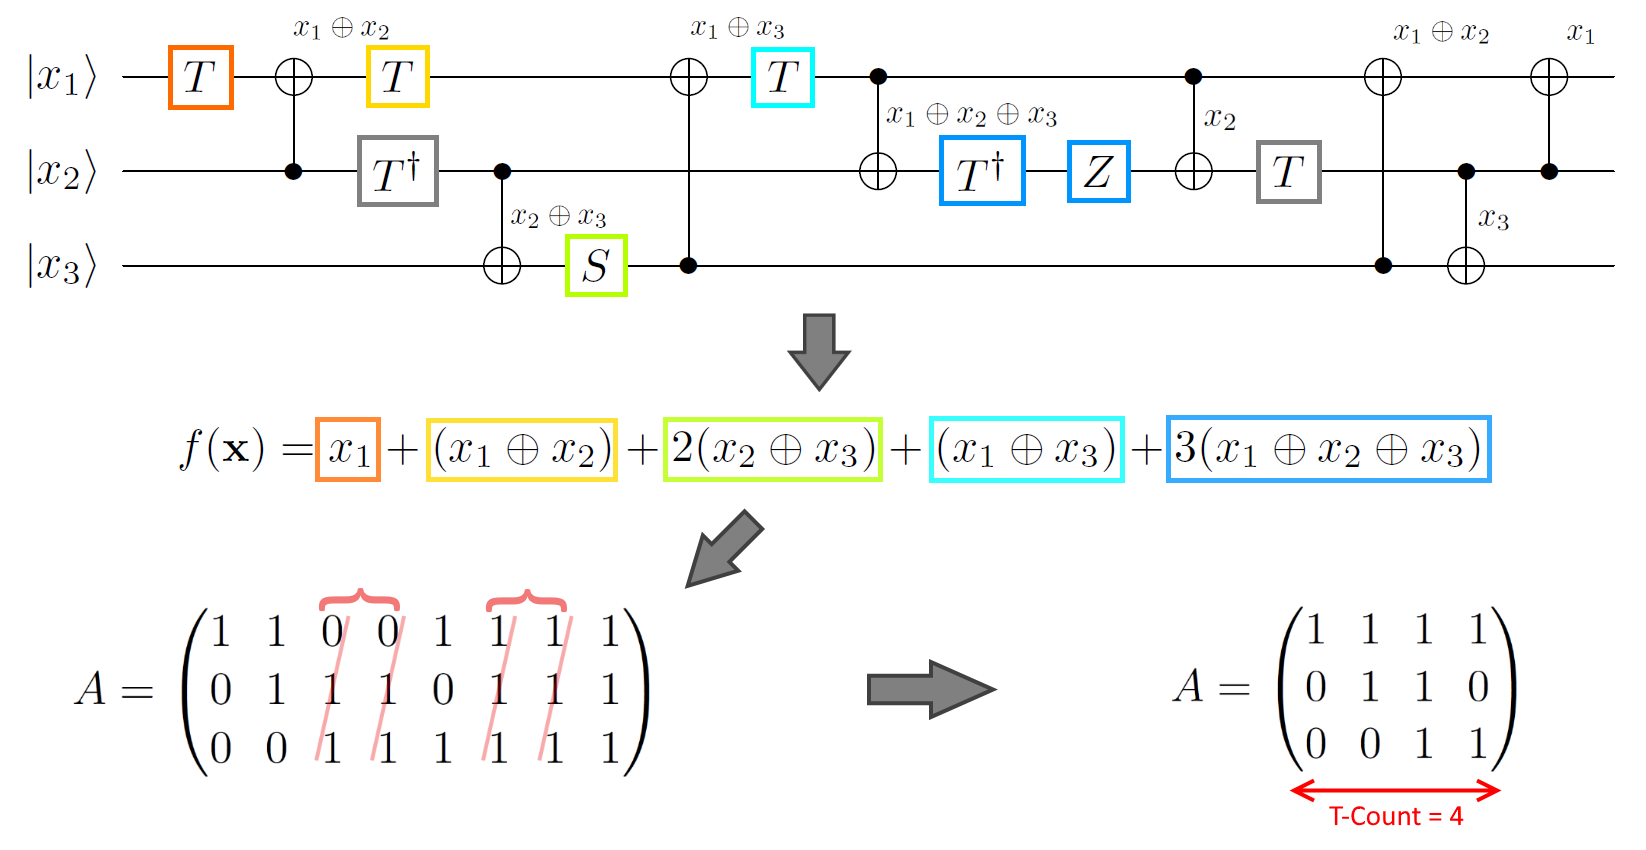
\includegraphics[width=\linewidth,cfbox=gray!75 1pt 1pt]{quant_circ1}
				\caption{Extracting a gate synthesis matrix from an example circuit.}
			\end{figure}
		\end{tcolorbox}

	\end{minipage}

	% RIGHT COLUMN
	
	\begin{minipage}[b]{0.95\linewidth}
		% UNIVERSAL CIRCUITS/APPENDIX
		\iffalse\begin{tcolorbox}[ title=\textcolor{white}{\huge\textbf{\textsf{Universal Circuits}\textcolor{black}{y}}}]
			Hadamard gadgets			
			\begin{figure}
				%\centering
				\begin{subfigure}{\textwidth}
					%\centering
					\includegraphics[width=0.5\textwidth]{hadamard}
				\end{subfigure}
				\begin{subfigure}{\textwidth}
					%\centering
					\includegraphics[width=0.5\textwidth]{toffoli}
				\end{subfigure}
			\end{figure}			
			Toffoli-n
		\end{tcolorbox}\fi

		% RESULTS FIGURE/RESULTS
		% RESULT SECTION/RESULTS
		\begin{tcolorbox}[title=\textcolor{white}{\huge\textbf{\textsf{Results}\textcolor{black}{y}}},left=0.5cm,right=0.5cm,top=0.5cm,bottom=0.5cm]
				
		
		\centering
		\begin{tcolorbox}[reset, colback=gray!75,colframe=black]
			\begin{figure}
				\centering
				%\begin{multicols}{2}
				\begin{subfigure}{0.45\textwidth}
					\centering
					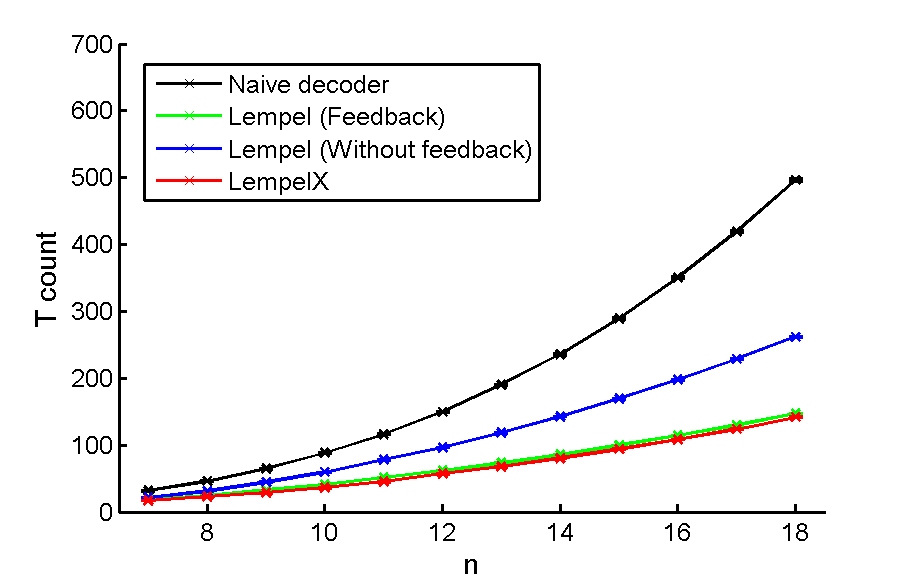
\includegraphics[width=\linewidth,frame]{LX_vs_Lempel}
					\subcaption{}
				\end{subfigure}\hspace{1cm}									
				\begin{subfigure}{0.47\textwidth}
					\centering
					\includegraphics[width=\linewidth,frame]{DeltaT}
					\subcaption{}
				\end{subfigure}
				%\end{multicols}		
				\caption*{\footnotesize Figure 2: Circuits generated by the $\mathrm{CNOT}$ and $T$ gate were randomly generated for varying number of qubits $n$ then optimized by our implementations of: \emph{LempelX}; \emph{Lempel}, based on \cite{1_Campbell_2017} and \cite{20_Lempel_1975}, and \emph{naive decoder} based on \cite{8_Amy_2016}. a) The average $T$-count for each $n$ over many random circuits are shown on the vertical axis. \emph{LempelX} produces circuit decompositions with the smallest $T$-counts on average but scales the same as the next best algorithm, \emph{Lempel}. Both of these algorithms are better than the naive decoder by a factor $n$. b) The difference between the $T$-counts for \emph{LempelX} and \emph{Lempel} converge on a constant $5.5\pm 0.7$ for large $n$.}
			\end{figure}
		\end{tcolorbox}
	
		\begin{tcolorbox}[reset,colback=gray!75,colframe=black,width=1\linewidth,top=0.05cm,bottom=0.7cm]
			\begin{figure}
				\footnotesize
				\centering				
				\iffalse \begin{tabularx}{\linewidth}{|X | r | r | r | r | r | r|}					
					\hline
					Circuit & $n_{\text{in}}$ & $n_{\text{out}}$ & $T_{\text{in}}$ & $T_{\text{out}}$ & $E_{\text{in}}$ & $E_{\text{out}}$ \\
					\hline
					\emph{$^\#$000F} & 5 & 5 & 7 & 5 & 3514 & 2528 \\
					\emph{$^\#$0001} & 6 & 39 & 40 & 21 & 20146 & 11206.5 \\
					\emph{$^\#$001F} & 6 & 39 & 43 & 22 & 21651 & 11773.5 \\
					\emph{$^\#$01} & 5 & 13 & 15 & 9 & 7536 & 4641 \\
					\emph{$^\#$1} & 3 & 3 & 7 & 5 & 3510 & 2516 \\
					\emph{$^\#$0003} & 6 & 6 & 15 & 7 & 7551 & 3698 \\
					\emph{$^\#$003} & 6 & 14 & 16 & 6 & 8057 & 3189 \\
					\emph{$^\#$03} & 4 & 8 & 7 & 5 & 3513 & 2565 \\
					\emph{$^\#$0007} & 6 & 64 & 47 & 13 & 23699 & 7310 \\
					\emph{$^\#$007F} & 6 & 27 & 40 & 19 & 20149 & 10235.5 \\
					\emph{$^\#$07} & 5 & 14 & 16 & 12 & 8044 & 6162.5 \\
					\emph{$^\#$013F} & 6 & 54 & 48 & 12 & 24192 & 7035 \\
					\emph{$^\#$0017} & 6 & 35 & 23 & 11 & 11606 & 6266.5 \\
					\emph{$^\#$017F} & 6 & 59 & 80 & 23 & 40279 & 12608.5 \\
					\emph{$^\#$17} & 4 & 10 & 7 & 5 & 3536 & 2615 \\
					\emph{$^\#$033F} & 5 & 6 & 7 & 5 & 3542 & 2559.5 \\
					\emph{$^\#$0117} & 6 & 116 & 79 & 13 & 39822 & 7855 \\
					\emph{$^\#$0356} & 5 & 6 & 12 & 6 & 6030 & 3073.5 \\
					\hline
				\end{tabularx}\fi
				\caption*{\footnotesize Table 1: $T$-counts for various universal Clifford + T benchmark circuits as synthesized by the extended Lempel algorithm are shown. $T_{\text{original}}$ are the best known results produced by the works cited in the \emph{Circuit} column, and $T_{\text{LempelX}}$ is the result for \emph{LempelX}. \textbf{$n_{\text{original}}$} is the number of qubits of the original circuit and \textbf{$n_{\text{out}}$} is the total number of qubits of the output circuit including ancillas used to implement multiply controlled Toffoli gates as well as Hadamards using path variables \cite{42_montanaro}. The total execution time in seconds for \emph{LempelX} run on an \emph{Intel i7} 2.40Gz processor is given in column \emph{Time}.}
				\begin{tabular}{ |>{\columncolor{white}}l|>{\columncolor{blue!25}}r|>{\columncolor{green!25}}r|>{\columncolor{gray!10}}r|>{\columncolor{white}}r|>{\columncolor{gray!10}}r|>{\columncolor{white}}r| }					
					\hline						
					\rowcolor{gray!25}
					\textbf{Circuit} & \textbf{$T_{\text{original}}$} & \textbf{$T_{\text{LempelX}}$} & \textbf{$T_{\text{naive}}$} & \textbf{$n_{\text{original}}$} & \textbf{$n_{\text{out}}$} & \textbf{Time (s)} \\
					\hline						
					hwb6\_47\_107 \cite{8_Amy_2016} & 71 & 55 & 102 & 6 & 43 & 91.713 \\
					hwb6-42-150 \cite{8_Amy_2016} & 71 & 46 & 140 & 6 & 43 & 160.198 \\
					nth\_prime6\_inc\_55\_667 \cite{8_Amy_2016} & 400 & 263 & 354 & 6 & 39 & 228.025 \\
					ham15-109-214 \cite{8_Amy_2016} & 97 & 28 & 65 & 15 & 47 & 27.756 \\
					ham15-70 \cite{8_Amy_2016} & 230 & 103 & 148 & 15 & 47 & 100.899 \\
					ham15tc1 \cite{8_Amy_2016} & 1019 & 258 & 359 & 15 & 50 & 270.862 \\
					\emph{$^\#$0117} \cite{41_soeken} & 79 & 13 & 63 & 6 & 116 & 118.64 \\
					\emph{$^\#$017F} \cite{41_soeken} & 80 & 23 & 59 & 6 & 59 & 20.618 \\
					\emph{$^\#$0001} \cite{41_soeken} & 40 & 21 & 46 & 6 & 39 & 5.2 \\
					\emph{$^\#$001F} \cite{41_soeken} & 43 & 22 & 55 & 6 & 39 & 4.382 \\
					\emph{$^\#$0007} \cite{41_soeken} & 47 & 13 & 31 & 6 & 64 & 10.141 \\
					\emph{$^\#$007F} \cite{41_soeken} & 40 & 19 & 46 & 6 & 27 & 1.267 \\
					\hline
				\end{tabular}			
			\end{figure}
		\end{tcolorbox}		
	\end{tcolorbox}
	
		% DISCUSSION AND CONCLUSIONS
		\begin{tcolorbox}[ title=\textcolor{white}{\huge\textbf{\textsf{Summary and Conclusions}\textcolor{black}{y}}}]
			\iffalse Computational efficiency of algorithm
			Asymptotic worst case limit (high order poly)
			In practice: execution times
			LempelX performs better on average than best known algorithms by a constant offset.
			LempelX has same worst case T count scaling with number of qubits as Reed-Muller/Lempel algorithms. Therefore qualifies as `near' optimal.
			Applications for exact synthesis of quantum circuits involving many qubits. \fi
			%
			We have presented a novel $T$-gate optimization algorithm that extends the principle of Lempel's factoring algorithm to symmetric tensors of order 3. This was benchmark tested on randomized  circuits composed of $\mathrm{CNOT}$ and $T$-gates, as well as structured Clifford + $T$ circuits and was found to perform better than the best known algorithms from previous works. The algorithm yields near-optimal solutions as the $T$-counts have the same scaling as optimal solutions of $\mathcal{O}(n^2)$. The algorithm is computationally efficient with worst-case execution times that scale asymptotically with the number of qubits as $\mathcal{O}(n^{14})$, compared to the super-polynomial scaling of $\mathcal{O}(2^{(2^n)})$ for optimal solvers. %For the universal circuits, a trade-off is revealed between the number of qubits and the $T$-count with the larger number of qubits due to the path variable \cite{42_montanaro} method of implementing Hadamards with the $\mathrm{CNOT}$ and $T$ gate set compatible with our algorithm.
		\end{tcolorbox}
		\begin{tcolorbox}[title=\textcolor{white}{\huge\textbf{\textsf{References\textcolor{black}{y}}}}]
			\renewcommand\refname{\vskip -2cm}
			\bibliography{keylit}
			\bibliographystyle{abbrv}
		\end{tcolorbox}
	\end{minipage}	
\end{multicols}
\iffalse\vspace{5cm}
\begin{multicols}{2}
	\begin{minipage}[t]{0.7\linewidth}	
		\begin{tcolorbox}[height=9cm,title=\textcolor{white}{\huge\textbf{\textsf{Acknowledgements\textcolor{black}{y}}}}]
			Some people

			Some more people
			
			Loads of people
		\end{tcolorbox}		
	\end{minipage}
	\begin{minipage}[t]{1.3\linewidth}	
		\begin{tcolorbox}[height=9cm,title=\textcolor{white}{\huge\textbf{\textsf{References\textcolor{black}{y}}}}]
			\renewcommand\refname{\vskip -2cm}
			\bibliography{ketlit}
			\bibliographystyle{abbrv}
		\end{tcolorbox}		
	\end{minipage}
\end{multicols}\fi

\end{document}